\documentclass[aps, reprint, amsmath, amssymb]{revtex4-1}

\usepackage{amsmath}
\usepackage{hhline}
\usepackage{float}
\usepackage{graphicx}
\usepackage[font=footnotesize,labelfont=bf]{caption}
\graphicspath{ {images/} }
\def\changemargin#1#2{\list{}{\rightmargin#2\leftmargin#1}\item[]}
\let\endchangemargin=\endlist 
\usepackage[artemisia]{textgreek}


\begin{document}
\title{A Comparison of Machine Learning Techniques for Classification of the Higgs Boson}
\author{Jared Moskowitz \& Julia Rowe}
\date{8 May 2015}

\maketitle

\section{Introduction}
One of the integral tasks of particle physics experiments is identifying elementary particles produced in high energy collisions. This can be especially problematic for the Higgs boson, given that the primary observed decay mode, W-W+, results in the production of quark jets, which are difficult to distinguish from the background. To help with this, supervised machine learning techniques are used for classification. These classification methods depend on the features of the particles predicted by the standard model.  Very large and noisy data is being dealt with, so speed and accuracy is of the utmost concern. The purpose of this analysis is to compare machine learning algorithms, looking at both the accuracy and how they scale with the number of features.  

\section{Methods}
Various algorithms from the Waikato Environment for Knowledge Analysis (WEKA) suite of machine learning software were tested under the same conditions. This suite was used because it is preinstalled on the Cluster super computer (the environment for running these tests) and seems to be popular in the data science community.  Learners were trained using Monte Carlo data and tested on real data from ATLAS.  Data was separated into four groups: even runs with nine features, odd runs with nine features, even runs with thirty-one features, and odd runs with thirty-one features.  These even and odd groups come from splitting our original training and test data in half so that we could run each algorithm twice on disjoint sets. Predictive machine models were built from each of these groups and were used to test the opposite group of runs with the same number of features.  

\subsection{The Algorithms}
\subsubsection{Decision Trees (c4.5)}
Decision trees recursively split on values of features based with priority of splits to those with the most information gain. This information gain can more specifically be represented with the equation:

\begin{equation}
\textrm{Gain} (\textrm{split}) = \textrm{Ent} (S) - \sum \limits_j \dfrac{|S_j|}{S} \textrm{Ent}(S_j)
\end{equation}

This equation corresponds to a change in entropy (metric of information) from one state to another. This is the change in entropy from Nodes represent decisions (make next decision on left child if energy greater that 126 GeV otherwise go right). The leaves represent binary classifications (signal or background). WEKA provides the c4.5 variation of this algorithm.

\subsubsection{Random Forest}
Random forests are made up of multiple decision trees using random feature selection and bootstrap aggregation to correct for the common problem of decision tree overfitting.  This algorithm creates multiple decision trees by selecting a smaller subset of the features and building trees. Our random forests created ten trees.  For runs with nine features each tree selected four of these features and for runs with thirty-one features six features were selected.

\subsubsection{Na{\"i}ve Bayes}
This algorithm creates simple probabilistic classifiers by applying Bayes' rule under the assumption of statistical independence between the features.  Although highly simplified, the Na{\"i"}ve Bayes algorithm has been successful in highly complex situations.  It is also highly scalable, making it an efficient algorithm.  

\subsubsection{Support Vector Machine}
Support vector machines builds a hyperplane that best separate the two categories of data. This hyperplane is defined by a subset of the training data called support vectors. The goal is to maximize the margin, which is the euclidean distance from a support vector to the hyperplane.  An advantage of SVMs is it uses a fixed number of support vectors from the sample, avoiding overfitting.  Often the data is projected into higher dimensional feature space, if the set is not separable in the given dimension.  The hyperplane is defined by the set of points \textbf{x} which satisfy the equation:

\begin{equation}
\mathbf{w} \cdot \mathbf{x} - b = 0
\end{equation}

where \textbf{w} is the vector normal to the hyperplane.  Anything above the hyperplane should have the label of 1 (signal) and anything below -1 (background).  

\section{Results}

\begin{table}[H]
  \begin{center}
    \caption{Accuracy of Cross Validation on Training Data} \label{tab:title} 
    \begin{tabular}{ | l || l | l | l | l |}
      \hline
      Algorithm & 9 Even & 9 Odd & 31 Even & 31 Odd \\ \hhline{|=||=|=|=|=|}
      Decision Tree & 88.41 \% & 87.98\% & 87.70\% & 87.75\% \\ \hline
      Random Forest & 88.72\% & 88.57\% &  88.82\% & 88.53\% \\ \hline
      Na{\"i}ve Bayes* & 87.52\% & 87.79\% & 84.94\% & 84.97\% \\ \hline
      SVM - linear & 87.07\% & 87.01\% & 87.33\% & 87.26\% \\ \hline
    \end{tabular}
  \end{center}
\end{table}

There is no significant difference in the cross validation accuracy with respect to the different algorithms.  Na{\"i}ve Bayes was the only one that showed a significant difference with respect to the number of features, which is expected as the assumption that the features are statistically independent worsen as the number of features increases.  From this data we do see the random forest slightly improved from the decision tree, although we do not have enough data to show if this is significant. 

\begin{table}[H]
  \begin{center}
    \caption{Area Under the ROC Curve} \label{tab:title} 
    \begin{tabular}{ | l || l | l | l | l |}
      \hline
      Algorithm & 9 Even & 9 Odd & 31 Even & 31 Odd \\ \hhline{|=||=|=|=|=|}
      Decision Tree & 0.907 & 0.904 & 0.855 & 0.861 \\ \hline
      Random Forest & 0.929 & 0.928  & 0.929  & 0.929 \\ \hline
      Na{\"i}ve Bayes* & 0.931  & 0.929 & 0.915 & 0.913 \\ \hline
      SVM - linear & 0.792 & 0.794 & 0.803 & 0.803 \\ \hline
    \end{tabular}
  \end{center}
  \begin{changemargin}{25px}{30px}
  \footnotesize{
  *Na{\"i}ve Bayes did not run cross-validation, so the even machines were tested on the odd training data and vice versa.}
  \end{changemargin}
\end{table}

The second performance metric recorded from the data is the AROC, the area under the Reciever Operating Characteristics curve, which is useful for comparing algorithms with different loss conditions. This is a standard measure of performance in classification experiments that corresponds to a graph with the TPrate on the vertical axis and the FPrate on the horizontal axis. The closer this number is to one, the more accurate the learner.  This supports the claim that the random forest improves upon the decision tree. This also shows that naives bayes is once again worse for more features.  Additionally this metric shows that decision trees are worse for more features.


\begin{table}[H]
  \begin{center}
    \caption{Time (in seconds) per Algorithm} \label{tab:title} 
    \begin{tabular}{ | l || l | l | l | l |}  
      \hline
      Algorithm & 9 Even & 9 Odd & 31 Even & 31 Odd \\ \hhline{|=||=|=|=|=|}
      Decision Tree & 10.056 & 8.605 & 26.672 & 29.490 \\ \hline
      Random Forest & 21.346 & 23.487 & 37.249 & 38.542 \\ \hline
      Na{\"i}ve Bayes & 1.381 & 1.687 & 2.989 & 3.099 \\ \hline
      SVM - linear & 17.110 & 17.572 & 86.40 & 82.086 \\ \hline
    \end{tabular}
  \end{center}
\end{table}

The time complexity of most algorithms scaled linearly or better with the number of features.  The exception to this is SVM, which had the worse time complexity. 

\begin{figure}[H]
    \centering
    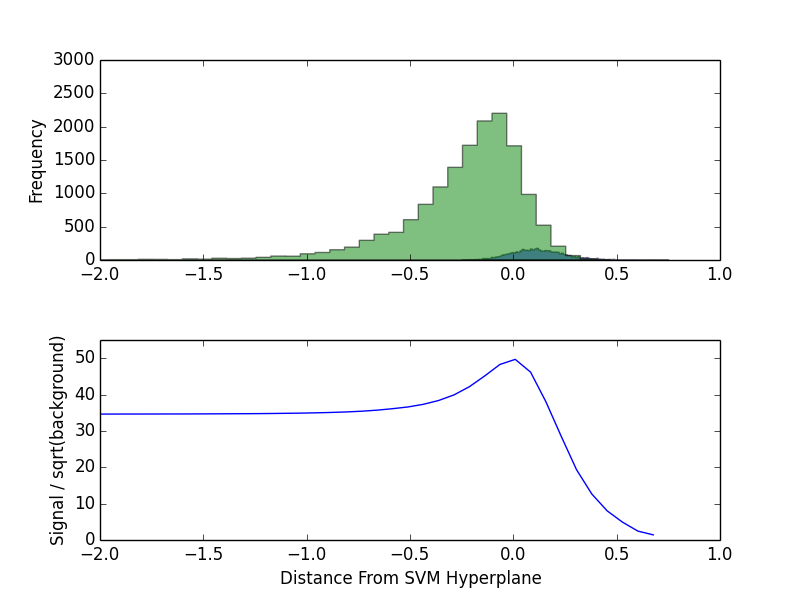
\includegraphics[width=\columnwidth]{signal-to-noise-9Even.png}
    \captionof{figure}{\textbf{a}. Light green shows the background while dark green shows the signal and their distances from the hyperplane, centered at 0.  \textbf{b}. Shows the signal to noise ratio defined as $\frac{s}{\sqrt{b}}$, where \textit{s} is signal and \textit{b} is background, as a function of a cut in the data, looking at data to the left of the cut.  Here we see the optimal cut is at 0 which is the location of the hyperplane. }
\end{figure}

SVM allows physical meaning from the data to be abstracted.  Separating the test data according to how it was classified shows the ratio of signal to background as a function of cut.  This give physical meaning to the error by showing the how the error changes with changes in the hyperplane.

\section{Conclusion}



\end{document}
